\documentclass[tikz,border=0pt]{standalone}
\usepackage{fontspec}
\hyphenpenalty=10000
\exhyphenpenalty=10000
\setmainfont[Path=../fonts/,BoldFont=Poppins-SemiBold.ttf,ItalicFont=Poppins-Italic.ttf]{Poppins-Regular.ttf}
\usepackage{pgfplots}
\pgfplotsset{compat=1.18}
\usetikzlibrary{calc,arrows.meta}
\definecolor{ink}{HTML}{161b22}
\definecolor{text}{HTML}{353535}
\definecolor{muted}{HTML}{646c74}
\definecolor{line}{HTML}{d7dadd}
\definecolor{wash}{HTML}{f6f6f6}
\definecolor{tint}{HTML}{e6ecef}
\definecolor{link}{HTML}{1d63b7}
\definecolor{local}{HTML}{376c97}
\definecolor{api}{HTML}{995d46}
\definecolor{cloud}{HTML}{7b649b}
\definecolor{match}{HTML}{7d9fc4}
\definecolor{miss}{HTML}{e0e3e5}
\definecolor{group}{HTML}{DCE2E5}
\definecolor{operation}{HTML}{C5CFD5}
\definecolor{mint}{HTML}{C9EEDF}
\definecolor{blueplane}{HTML}{AEC8E0}
\definecolor{pinkplane}{HTML}{F6D5DE}
\definecolor{peachplane}{HTML}{FFDBB8}
\definecolor{purpleplane}{HTML}{DCC7E7}
\begin{document}
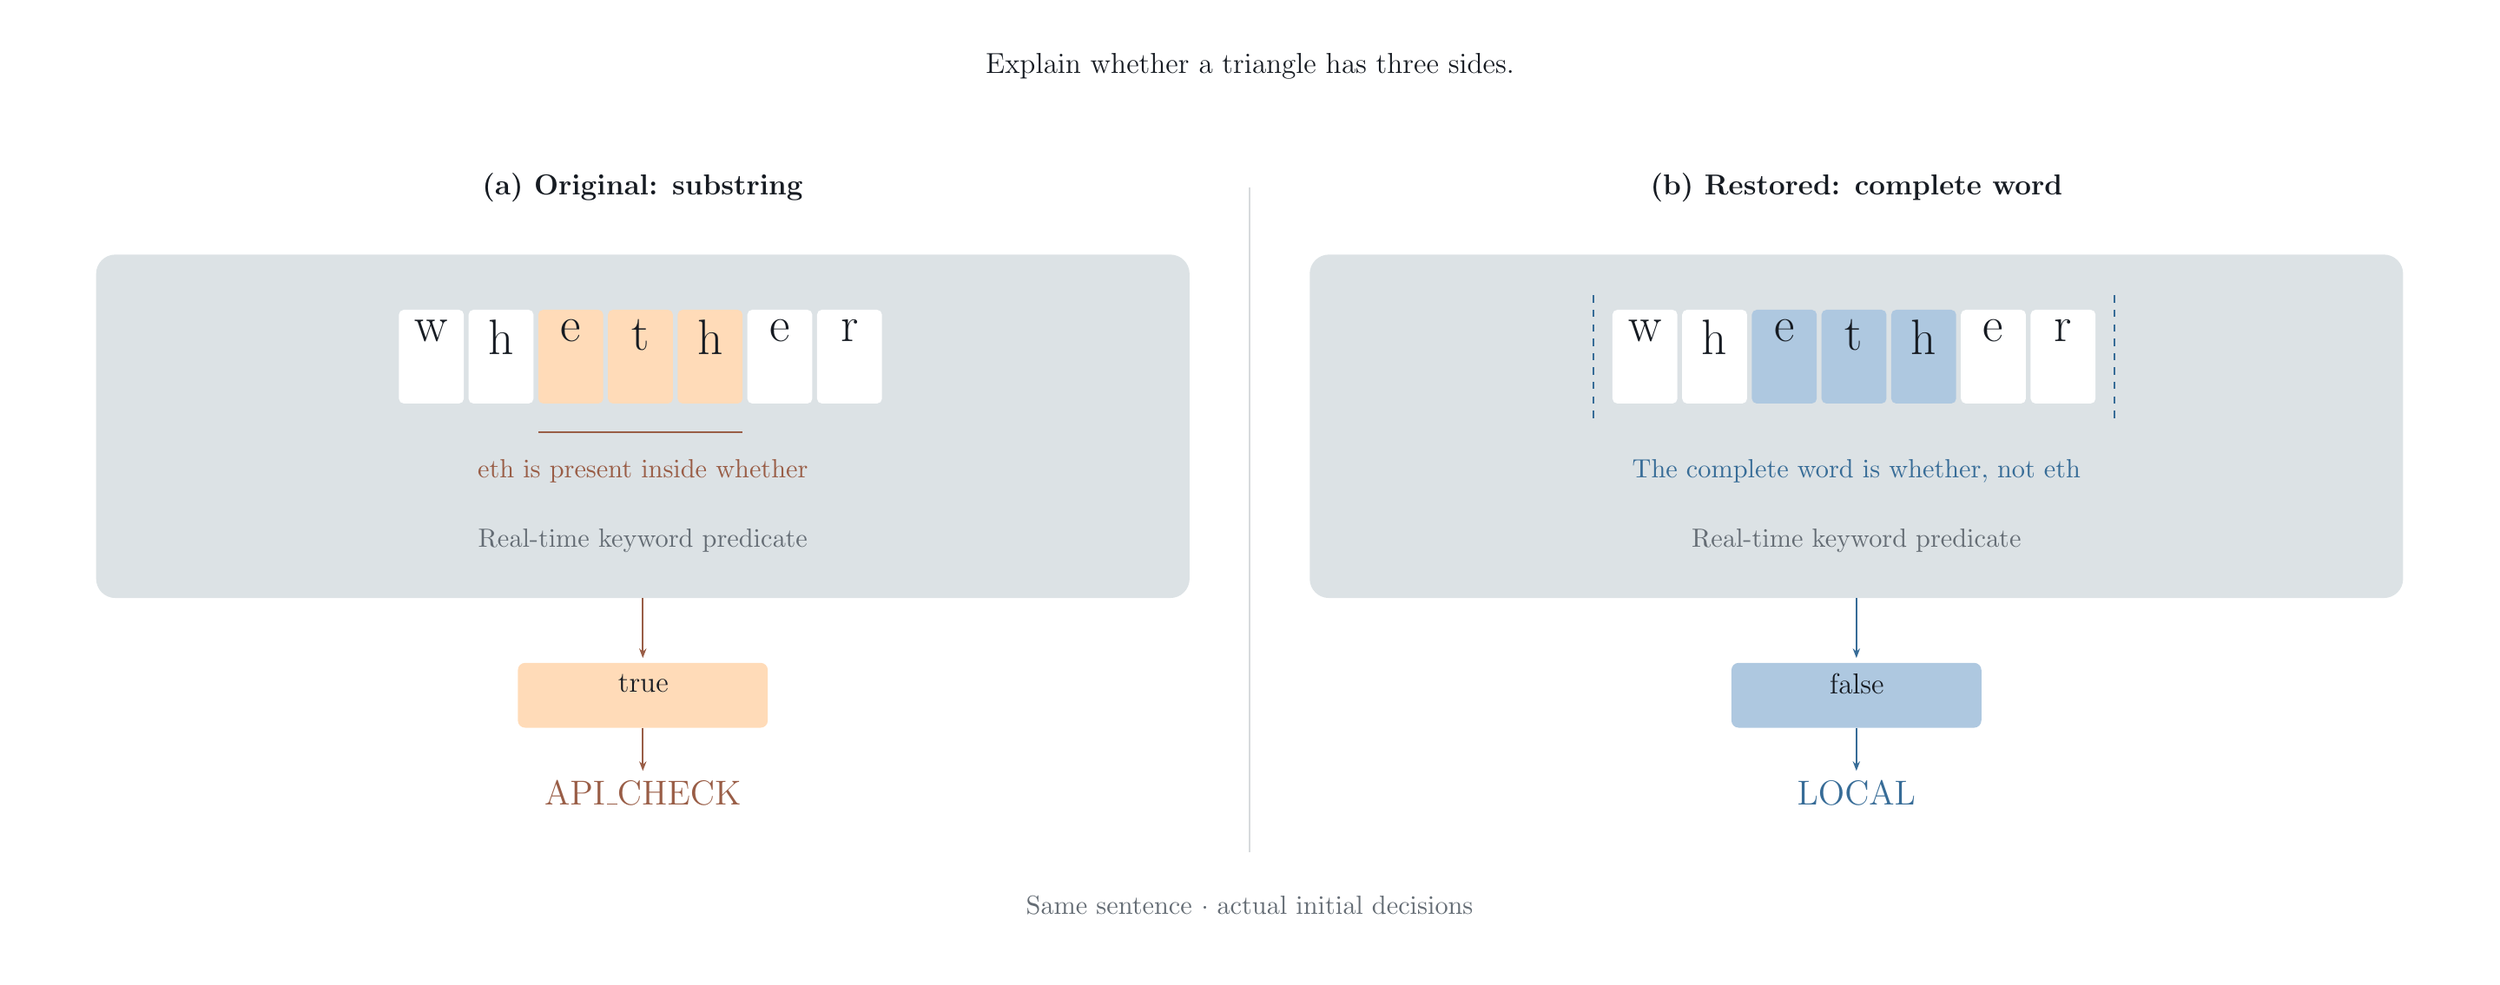
\begin{tikzpicture}[x=1pt,y=-1pt]
\path[use as bounding box] (0,0) rectangle (1020,390);
\node[anchor=north west,inner sep=0pt,text=ink,align=center,font=\fontsize{13}{19.5}\selectfont,text width=988pt] at (16.0,12) {Explain whether a triangle has three sides.};
\node[anchor=north west,inner sep=0pt,text=ink,align=center,font=\fontsize{13}{19.5}\selectfont,anchor=north] at (257.5,62) {\textbf{(a) Original: substring}};
\path[fill=group,rounded corners=8pt] (30,96) rectangle (485,239);
\path[fill=white,rounded corners=2pt] (156.0,119) rectangle (183.0,158);
\node[anchor=north west,inner sep=0pt,text=ink,align=center,font=\fontsize{22}{33.0}\selectfont,anchor=north] at (169.5,123) {w};
\path[fill=white,rounded corners=2pt] (185.0,119) rectangle (212.0,158);
\node[anchor=north west,inner sep=0pt,text=ink,align=center,font=\fontsize{22}{33.0}\selectfont,anchor=north] at (198.5,123) {h};
\path[fill=peachplane,rounded corners=2pt] (214.0,119) rectangle (241.0,158);
\node[anchor=north west,inner sep=0pt,text=ink,align=center,font=\fontsize{22}{33.0}\selectfont,anchor=north] at (227.5,123) {e};
\path[fill=peachplane,rounded corners=2pt] (243.0,119) rectangle (270.0,158);
\node[anchor=north west,inner sep=0pt,text=ink,align=center,font=\fontsize{22}{33.0}\selectfont,anchor=north] at (256.5,123) {t};
\path[fill=peachplane,rounded corners=2pt] (272.0,119) rectangle (299.0,158);
\node[anchor=north west,inner sep=0pt,text=ink,align=center,font=\fontsize{22}{33.0}\selectfont,anchor=north] at (285.5,123) {h};
\path[fill=white,rounded corners=2pt] (301.0,119) rectangle (328.0,158);
\node[anchor=north west,inner sep=0pt,text=ink,align=center,font=\fontsize{22}{33.0}\selectfont,anchor=north] at (314.5,123) {e};
\path[fill=white,rounded corners=2pt] (330.0,119) rectangle (357.0,158);
\node[anchor=north west,inner sep=0pt,text=ink,align=center,font=\fontsize{22}{33.0}\selectfont,anchor=north] at (343.5,123) {r};
\draw[draw=api,line width=.7pt] (214.0,170) -- (299.0,170);
\node[anchor=north west,inner sep=0pt,text=api,align=center,font=\fontsize{11}{16.5}\selectfont,anchor=north] at (257.5,181) {eth is present inside whether};
\node[anchor=north west,inner sep=0pt,text=muted,align=center,font=\fontsize{10.5}{15.75}\selectfont,anchor=north] at (257.5,210) {Real-time keyword predicate};
\draw[-{Stealth[length=4pt,width=3pt]},draw=api,line width=.7pt] (257.5,239) -- (257.5,264);
\path[fill=peachplane,rounded corners=3pt] (205.5,266) rectangle (309.5,293);
\node[anchor=north west,inner sep=0pt,text=ink,align=center,font=\fontsize{12}{18.0}\selectfont,text width=96pt] at (209.5,270.5) {true};
\draw[-{Stealth[length=4pt,width=3pt]},draw=api,line width=.7pt] (257.5,293) -- (257.5,311);
\node[anchor=north west,inner sep=0pt,text=api,align=center,font=\fontsize{15}{22.5}\selectfont,anchor=north] at (257.5,315) {API\_CHECK};
\node[anchor=north west,inner sep=0pt,text=ink,align=center,font=\fontsize{13}{19.5}\selectfont,anchor=north] at (762.5,62) {\textbf{(b) Restored: complete word}};
\path[fill=group,rounded corners=8pt] (535,96) rectangle (990,239);
\path[fill=white,rounded corners=2pt] (661.0,119) rectangle (688.0,158);
\node[anchor=north west,inner sep=0pt,text=ink,align=center,font=\fontsize{22}{33.0}\selectfont,anchor=north] at (674.5,123) {w};
\path[fill=white,rounded corners=2pt] (690.0,119) rectangle (717.0,158);
\node[anchor=north west,inner sep=0pt,text=ink,align=center,font=\fontsize{22}{33.0}\selectfont,anchor=north] at (703.5,123) {h};
\path[fill=blueplane,rounded corners=2pt] (719.0,119) rectangle (746.0,158);
\node[anchor=north west,inner sep=0pt,text=ink,align=center,font=\fontsize{22}{33.0}\selectfont,anchor=north] at (732.5,123) {e};
\path[fill=blueplane,rounded corners=2pt] (748.0,119) rectangle (775.0,158);
\node[anchor=north west,inner sep=0pt,text=ink,align=center,font=\fontsize{22}{33.0}\selectfont,anchor=north] at (761.5,123) {t};
\path[fill=blueplane,rounded corners=2pt] (777.0,119) rectangle (804.0,158);
\node[anchor=north west,inner sep=0pt,text=ink,align=center,font=\fontsize{22}{33.0}\selectfont,anchor=north] at (790.5,123) {h};
\path[fill=white,rounded corners=2pt] (806.0,119) rectangle (833.0,158);
\node[anchor=north west,inner sep=0pt,text=ink,align=center,font=\fontsize{22}{33.0}\selectfont,anchor=north] at (819.5,123) {e};
\path[fill=white,rounded corners=2pt] (835.0,119) rectangle (862.0,158);
\node[anchor=north west,inner sep=0pt,text=ink,align=center,font=\fontsize{22}{33.0}\selectfont,anchor=north] at (848.5,123) {r};
\draw[draw=local,line width=.7pt,dashed] (653.0,113) -- (653.0,164);
\draw[draw=local,line width=.7pt,dashed] (870.0,113) -- (870.0,164);
\node[anchor=north west,inner sep=0pt,text=local,align=center,font=\fontsize{10.7}{16.049999999999997}\selectfont,anchor=north] at (762.5,181) {The complete word is whether, not eth};
\node[anchor=north west,inner sep=0pt,text=muted,align=center,font=\fontsize{10.5}{15.75}\selectfont,anchor=north] at (762.5,210) {Real-time keyword predicate};
\draw[-{Stealth[length=4pt,width=3pt]},draw=local,line width=.7pt] (762.5,239) -- (762.5,264);
\path[fill=blueplane,rounded corners=3pt] (710.5,266) rectangle (814.5,293);
\node[anchor=north west,inner sep=0pt,text=ink,align=center,font=\fontsize{12}{18.0}\selectfont,text width=96pt] at (714.5,270.5) {false};
\draw[-{Stealth[length=4pt,width=3pt]},draw=local,line width=.7pt] (762.5,293) -- (762.5,311);
\node[anchor=north west,inner sep=0pt,text=local,align=center,font=\fontsize{15}{22.5}\selectfont,anchor=north] at (762.5,315) {LOCAL};
\draw[draw=line,line width=.7pt] (510,68) -- (510,345);
\node[anchor=north west,inner sep=0pt,text=muted,align=center,font=\fontsize{10.5}{15.75}\selectfont,anchor=north] at (510.0,363) {Same sentence · actual initial decisions};

\end{tikzpicture}
\end{document}
